\documentclass{article}

\usepackage{amsmath,amssymb,amsthm,graphicx}
\usepackage{subcaption}
\usepackage{float}

\setlength{\oddsidemargin}{0.25 in}
\setlength{\evensidemargin}{-0.25 in}
\setlength{\topmargin}{-0.6 in}
\setlength{\textwidth}{6.5 in}
\setlength{\textheight}{8.5 in}
\setlength{\headsep}{0.75 in}
\setlength{\parindent}{0 in}
\setlength{\parskip}{0.1 in}

\newtheorem{theorem}{Theorem}
\newtheorem{corollary}{Corollary}
\newtheorem{proposition}{Proposition}
\newtheorem*{remark}{Remark}
\theoremstyle{definition}
\newtheorem{example}{Example}
\newtheorem{definition}{Definition}

\newcommand{\lecture}[4]{
   \pagestyle{myheadings}
   \thispagestyle{plain}
   \newpage
%   \setcounter{lecnum}{#1}
   \setcounter{page}{1}
   \noindent
   \begin{center}
   \framebox{
      \vbox{\vspace{2mm}
    \hbox to 6.58in { {\bf CSC~565: Graph Theory
                        \hfill North Carolina State University} }
    \hbox to 6.58in { {\bf Fall 2019
                        \hfill Computer Science} }
       \vspace{4mm}
       \hbox to 6.28in { {\Large \hfill Lecture #1: #2  \hfill} }
       \vspace{2mm}
       \hbox to 6.28in { {\it Lecturer: {\it Don Sheehy {\tt <drsheehy@ncsu.edu>}} \hfill Scribe: #4} }
      \vspace{2mm}}
   }
   \end{center}
   \markboth{Lecture #1: #2}{Lecture #1: #2}
   \vspace*{4mm}
}


\begin{document}
    \lecture{19}{Oct 28, 2019}{}{Calvin Nguyen, Niharika Acharya, Shreeya Singh Dhakal}
    
    \section{Overview}
    In this lecture we discussed Maxwell-Cremona correspondence and projections of planar graphs to 3-D spaces. We also looked into liftings, reciprocal diagrams, equilibrium stress and correspondences between them. In this lecture we are considering planar, 3-connected graphs, which make an important class of graphs in graph theory because for 3-connected graphs, you will get same set of faces regardless of how you draw it.
    
    
    
    
    \section{Review}
    In this section we will briefly define concepts that are important to fully understand the concepts taught in this and next lectures(Lecture 19 and 20).
    
    \textbf{Polytopal Graphs:} Polytopal graphs are planar, 3-connected graphs formed by edges and vertices of convex polytopes. 
    
    \textbf{Platonic Solids:} A platonic solid is a regular, convex polyhedron that can be defined algebraically as the set of solutions to a system of linear inequalities. There are exactly five platonic solids: tetrahedron, cube, 	octahedron, dodecahedron and icosahedron.
    
    \textbf{Monotone Paths:} A monotone path in a graph is a straight line drawing such that for every edge there exists a monotonically increasing path in some direction.
    
    \textbf{Planar Graphs and Duals:} A planar graph is a graph that can be drawn on a plane without an edge crossing. A complete graph on 4 vertices, ${K_4}$, is an example of such graph.
    
    \begin{figure}[H]
        \centering
        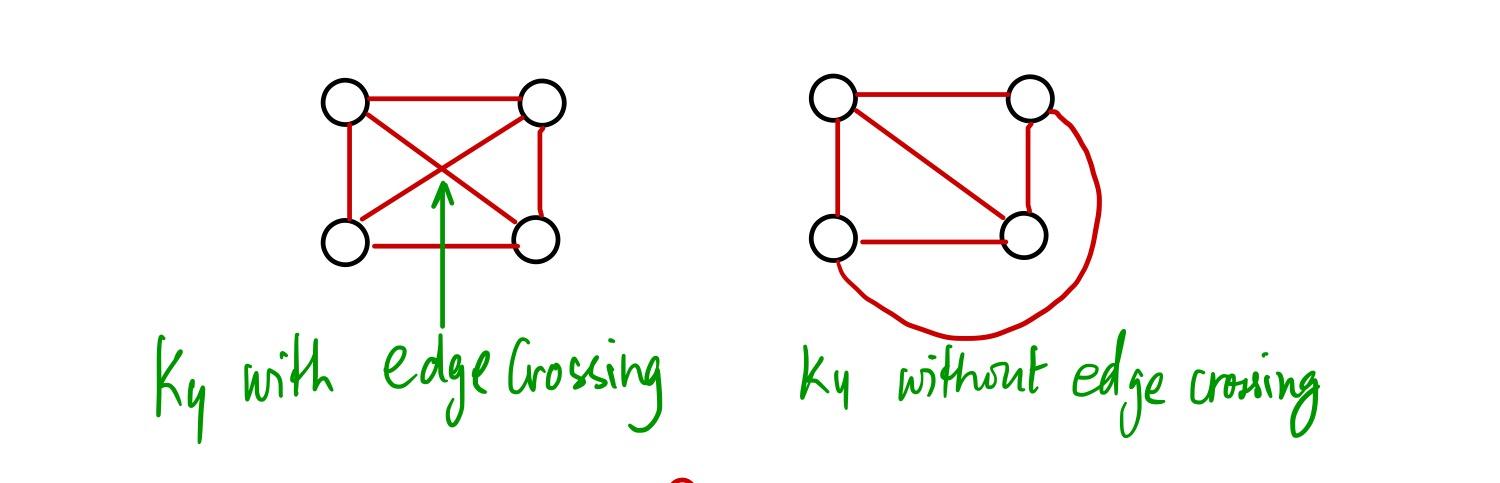
\includegraphics[width=.6\linewidth]{planar.JPG}
        \caption{Example of a planar graph}
        \label{fig:planar-graph}
    \end{figure}
    
    A dual of a plane graph $G$, is a graph that has a vertex for each face in G and an edge for each pair of faces separated by a common edge.
    \begin{figure}[H]
        \centering
        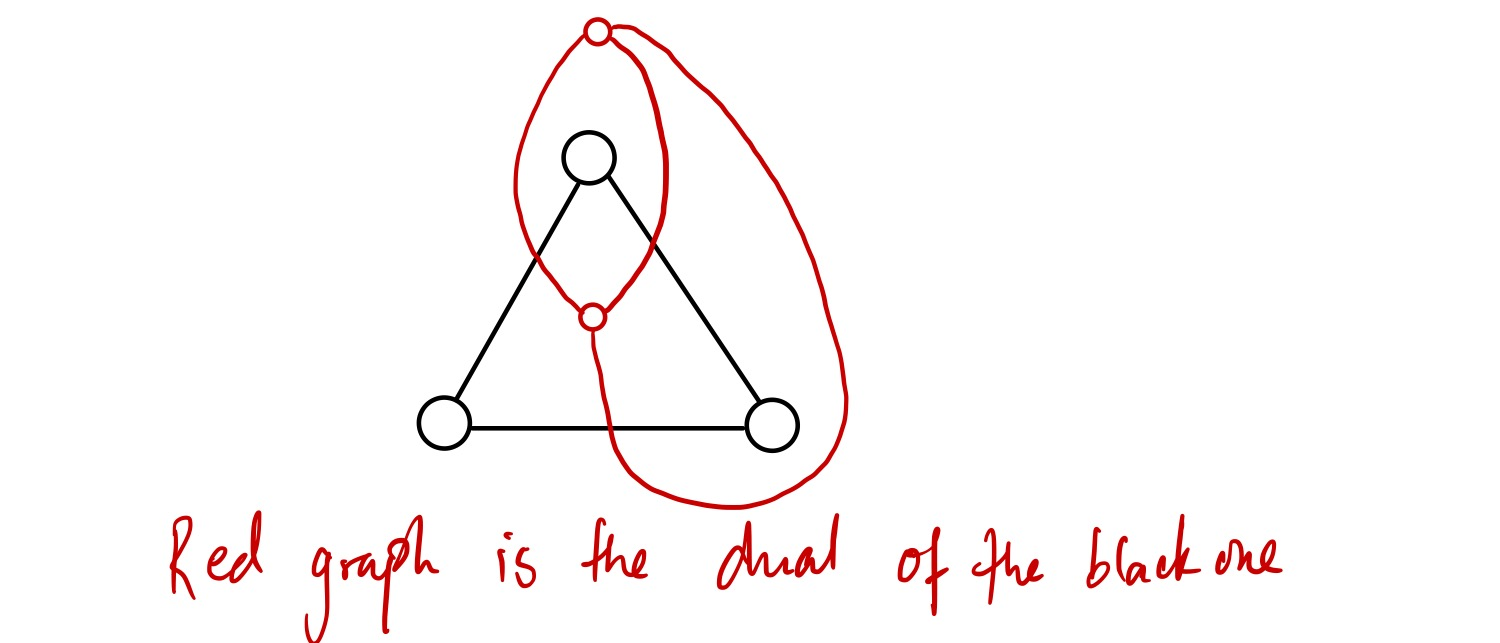
\includegraphics[width=.5\linewidth]{dual-example.JPG}
        \caption{Example of a graph dual}
        \label{fig:dual-example}
    \end{figure}
    
    \textbf{Linear embeddings of graphs:} In linear embeddings of graphs, vertices are chosen from the interval $[0, 1]$ and edges are chosen such that for every vertex, \textit{'v'} in the graph the probability of an edge to y decreases with the increasing distance between x and y.
    
    \textbf{Lifting:} A lifting of a straight-line drawing of a planar graph is an assignment of heights to vertices such that all faces stay co-planar in ${\rm I\!R^3}$. 
    
    \textbf{Equilibrium stress:} An equilibrium stress on a straight-line drawing of a graph is stress such that the sum of push and pull along the lines incident on each vertex is zero.
    
    \textbf{Reciprocal Diagrams:} A reciprocal diagram is a kind of planar graph duals. A reciprocal diagram of a diagram represented by points acted on by some force along the lines incident on the points is a closed polygon formed by corresponding lines of forces in the primal graph. Figure 3 shows an example of a force diagram and its dual closed polygon/reciprocal diagram.
    
    \begin{figure}[H]
        \centering
        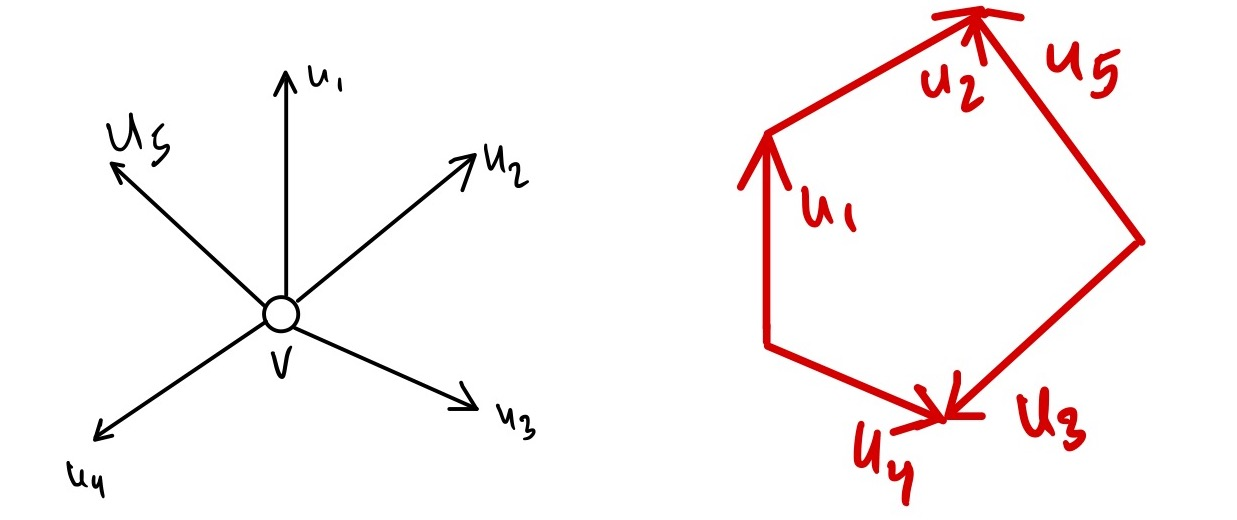
\includegraphics[width=.65\linewidth]{reciprocal.JPG}
        \caption{Example of reciprocal diagrams}
        \label{fig:dual-example}
    \end{figure}
    
    
    \section{Maxwell-Cremona Correspondence}

    
    Given a force diagram, is there a way to show that the net force is zero?
    
    In a force diagram, an equilibrium can be identified by "glueing" all the forces together to a polygon; aptly named the reciprocal diagram. In graph theoretic terms, Maxwell was attempting to create a linear drawing of the dual of a force diagram.
    
    We will only deal with planar, 3-connected graphs; these kinds of graphs satisfy the intuitive sense of dual where applying the dual operation twice results in the same starting graph.
    
    \begin{corollary}[]
        Given a graph $G$ which is planar and 3-connected, then the dual graph can be constructed as follows $G^*=(F_G, \{(A,B): A,B \text{ faces sharing an edge} \}$.
    \end{corollary}
    
    \begin{remark}[]
        Sticking to a planar, 3-connected graph yields cycles that always apply to the same faces.
    \end{remark}
    
    \begin{remark}[]
        At least two faces that can meet at any edge.
    \end{remark}
    
    \begin{remark}
        There is one edge in the dual graph for every edge in the primal graph.
    \end{remark}
    
    Maxwell's Correspondence poses a more general question, it is for any graph $G$, give a linear drawing of $G^*$ showing that the edges are parallel.
    
    For example, given the force diagram (a), we would like to construct (b).
    
    \begin{figure}[H]
    \centering
        \begin{subfigure}{.4\textwidth}
            \centering
            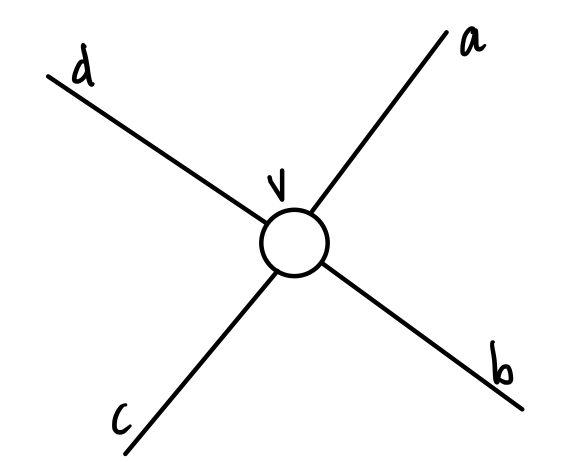
\includegraphics[width=.5\linewidth]{force_diagram.jpeg}
            \caption{$\underbar{G}$: a force diagram}
        \end{subfigure}%
        \begin{subfigure}{.4\textwidth}
            \centering
            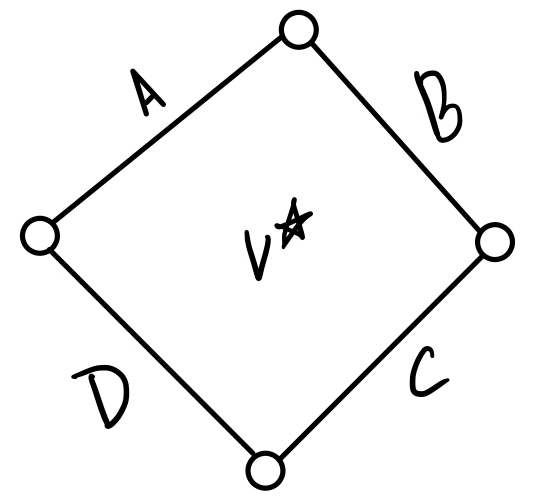
\includegraphics[width=.5\linewidth]{reciprocal_diagram.jpeg}
            \caption{$\underbar{G}^*$: the reciprocal of the force diagram}
        \end{subfigure}
    \end{figure}
    
    There exists another way to draw the reciprocal diagram, instead of drawing the edges in parallel, draw them perpendicular. Meaning a$\bot$A, b$\bot$B, and so on.
    
    \begin{remark}
        Any force diagram with more than $2n-3$ edges causes problems in drawing the reciprocal, meaning Maxwell's Correspondence fails for truly random edges.
        
        But, that won't happen since the directions all come from another graph.
    \end{remark}
    
    
    The smallest example of this would be a $K_4$,
    
    \begin{figure}[H]
    \centering
        \begin{subfigure}{.4\textwidth}
            \centering
            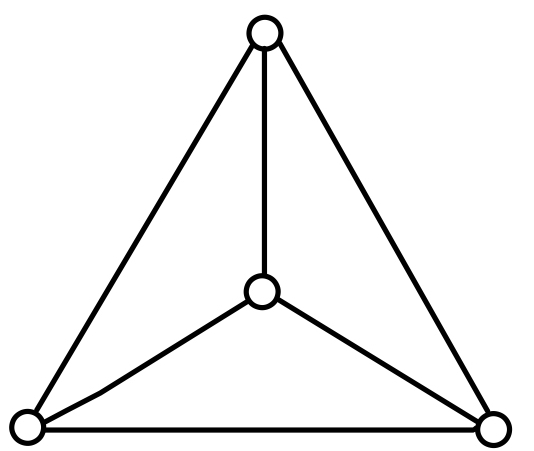
\includegraphics[width=.5\linewidth]{k_4.jpeg}
            \caption{$\underbar{G}$: a $K_4$ force diagram}
        \end{subfigure}%
        \begin{subfigure}{.4\textwidth}
            \centering
            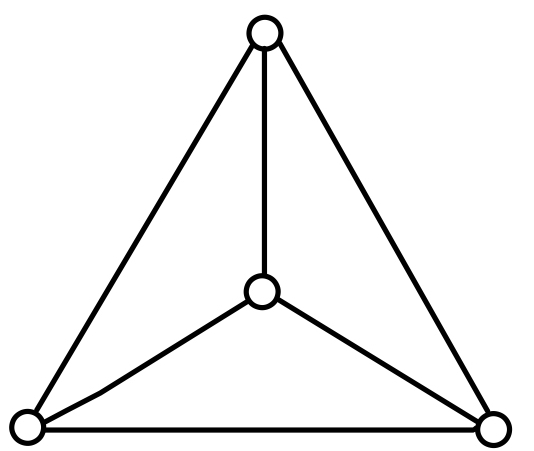
\includegraphics[width=.48\linewidth, angle=180]{k_4.jpeg}
            \caption{$\underbar{G}^*$: the reciprocal of the force diagram}
        \end{subfigure}
    \end{figure}
    
    But the reciprocal diagram wouldn't be its dual graph, but where the edges are orthogonal to each other.
    
    A 3-connected graph on 5 vertices example would be $K_5$ minus one edge, it is also minimally non-planar.
    
    For the graph $G$,
    
    \begin{figure}[h!]
            \centering
            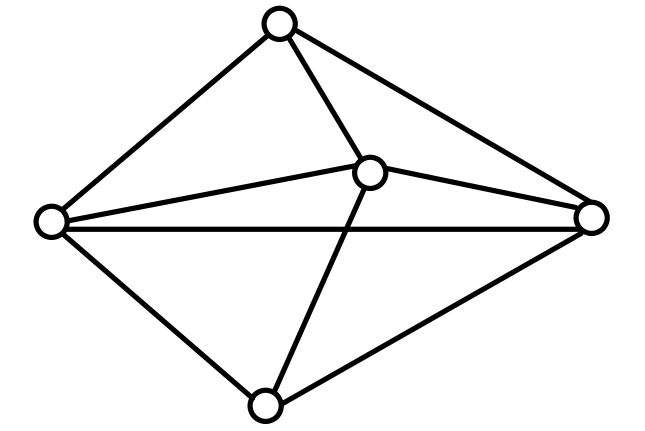
\includegraphics[width=.3\linewidth]{fake_k5.jpeg}
            \caption{$\underbar{G}$: a $K_5$ with one missing edge}
    \end{figure}
    
    \begin{align}
        |V_G| &= 5 \\
        |E_G| &= 9 \\
        |F_G| &= 6
    \end{align}
    
    then the dual $G^*$ would be something more \textit{regular},
    
    \begin{figure}[H]
        \centering
        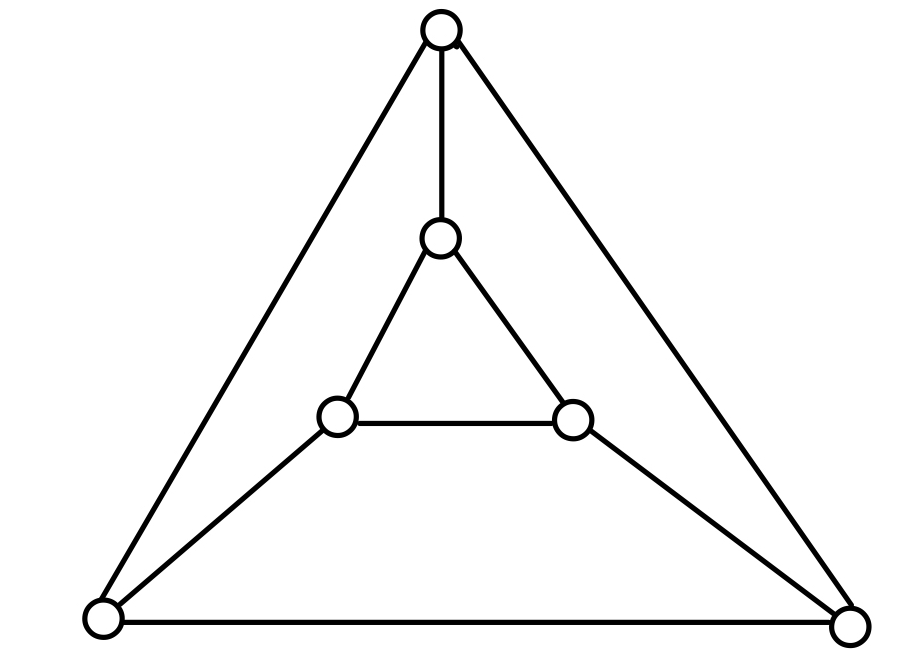
\includegraphics[width=.3\linewidth]{fake_k5_recip.jpeg}
        \caption{$\underbar{G}$$^*$: The dual of G}
    \end{figure}
    
     \begin{align}
        |V_G| &= 6 \\
        |E_G| &= 9 \\
        |F_G| &= 5
    \end{align}
    
    \begin{remark}
        The degree 4 vertices would turn into quadrilaterals in the dual.
    \end{remark}
    
    This leads into the idea that what Maxwell wanted to draw were just projections into 3D.
    
    \section{Projections to 3D}
    
    To lift objects in $\mathbb{R}^2$ to $\mathbb{R}^3$, define the following terminology first.
    
    \begin{definition}
        A point in the plane, $p \in \mathbb{R}^2$.
    \end{definition}
    
    \begin{definition}
        A point in 3D space, $\hat{p}=
        \begin{bmatrix}
        p \\
        p_z
        \end{bmatrix} \in \mathbb{R}^3$.
    \end{definition}
    
    \begin{definition}
        A linear function where the graph of it will be a plane, $f(p) \in \mathbb{R}$
    \end{definition}
    
    \begin{definition}
        A plane defined as $\hat{p}^* = \{ \begin{bmatrix}
        p \\
        p_z
        \end{bmatrix} \in \mathbb{R}^3: x_z=p^Tx-p_z \}$ which is the set of all points in the plane, where $p$ is the gradient.
    \end{definition}
    
    We want to be able to switch between a plane and a point.
    
    \begin{corollary}[]
        $\hat{p} \in \hat{q}^*$ if and only if $\hat{q} \in \hat{p}^*$.
    \end{corollary}
    
    \begin{figure}[H]
        \centering
        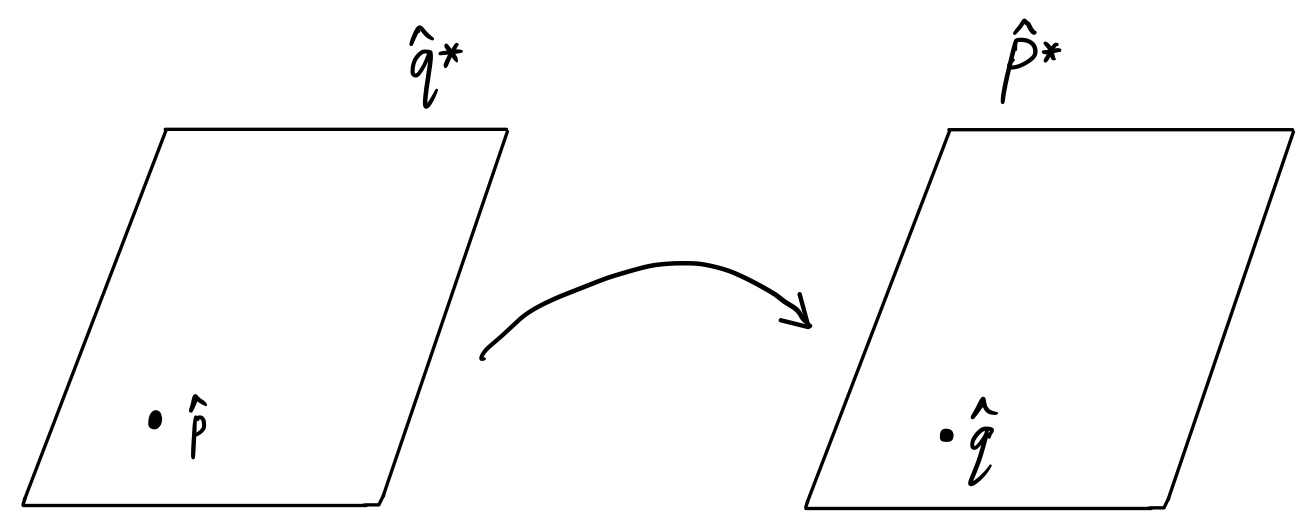
\includegraphics[width=.5\linewidth]{conversion.jpeg}
        \caption{Find a point in a plane means swapping object types hold the encapsulation.}
    \end{figure}
    
    \begin{proof}
        Given $\hat{q} \in \hat{p}^*$, that means $q_z=p^Tq-p_z$; therefore $p_z=p^Tq-q_z$. Concluding $\hat{p} \in \hat{q}^*$.
        
        Given $\hat{p} \in \hat{q}^*$, apply Definition 4 but swap $x$ for $q$.
    \end{proof}
    
    \begin{definition}[lifting]
        A \textbf{lifting} of a planar drawing is an assignment of heights to vertices so that faces stay coplanar.
    \end{definition}
    
    \begin{remark}
        Given a lifting, there is a plane $\hat{q}^*$ for every face.
    \end{remark}
    

    
    The reciprocal diagram will draw the face as point $q$.
    
    \begin{figure}[H]
        \centering
        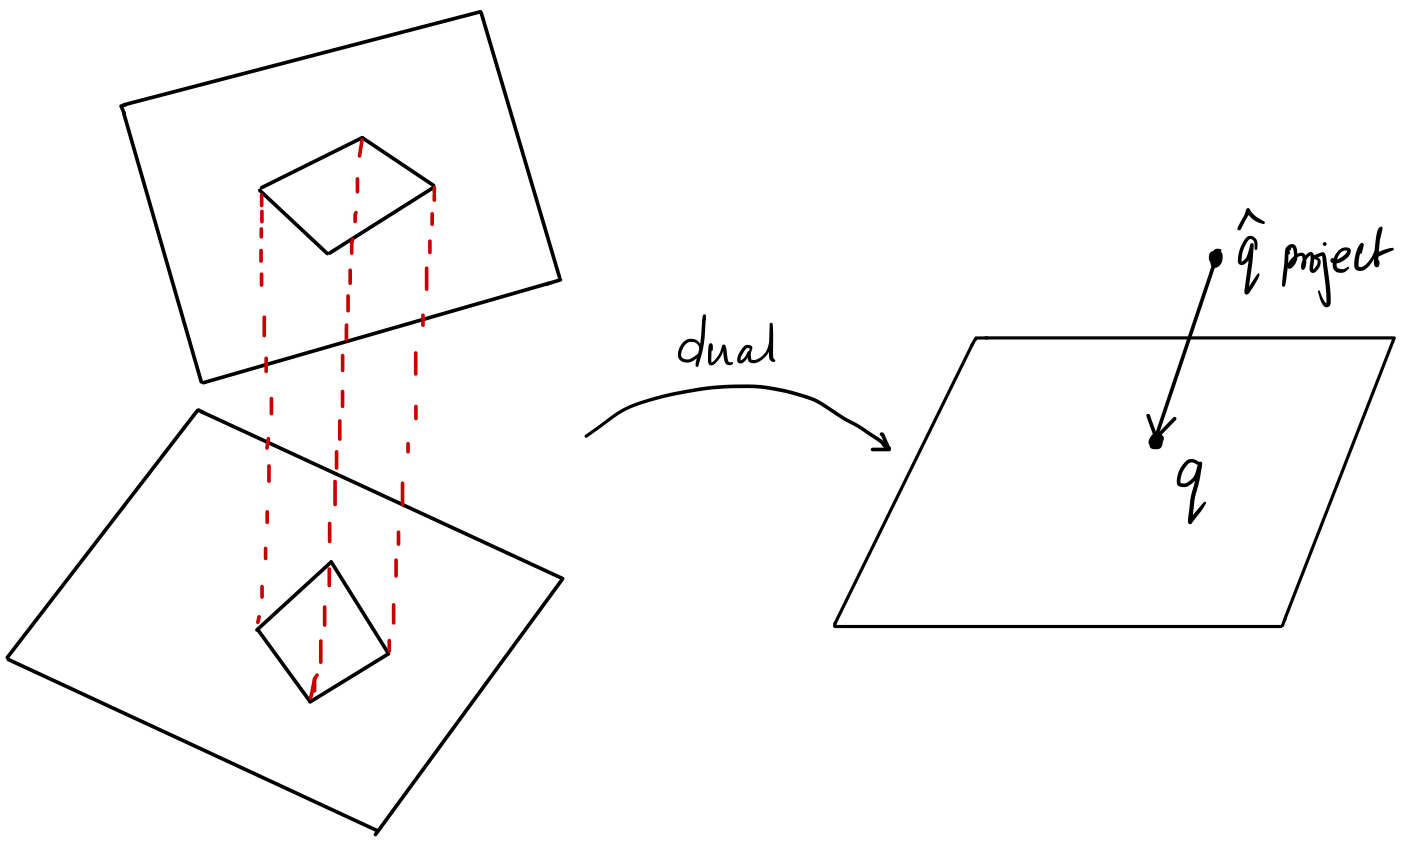
\includegraphics[width=.5\linewidth]{dual.jpeg}
        \caption{Conversion of a face to a point.}
    \end{figure}
    
    What happens to a $P_2$ after a lifting? Two new planes intersect each other forming a line.
    
    \begin{figure}[H]
        \centering
        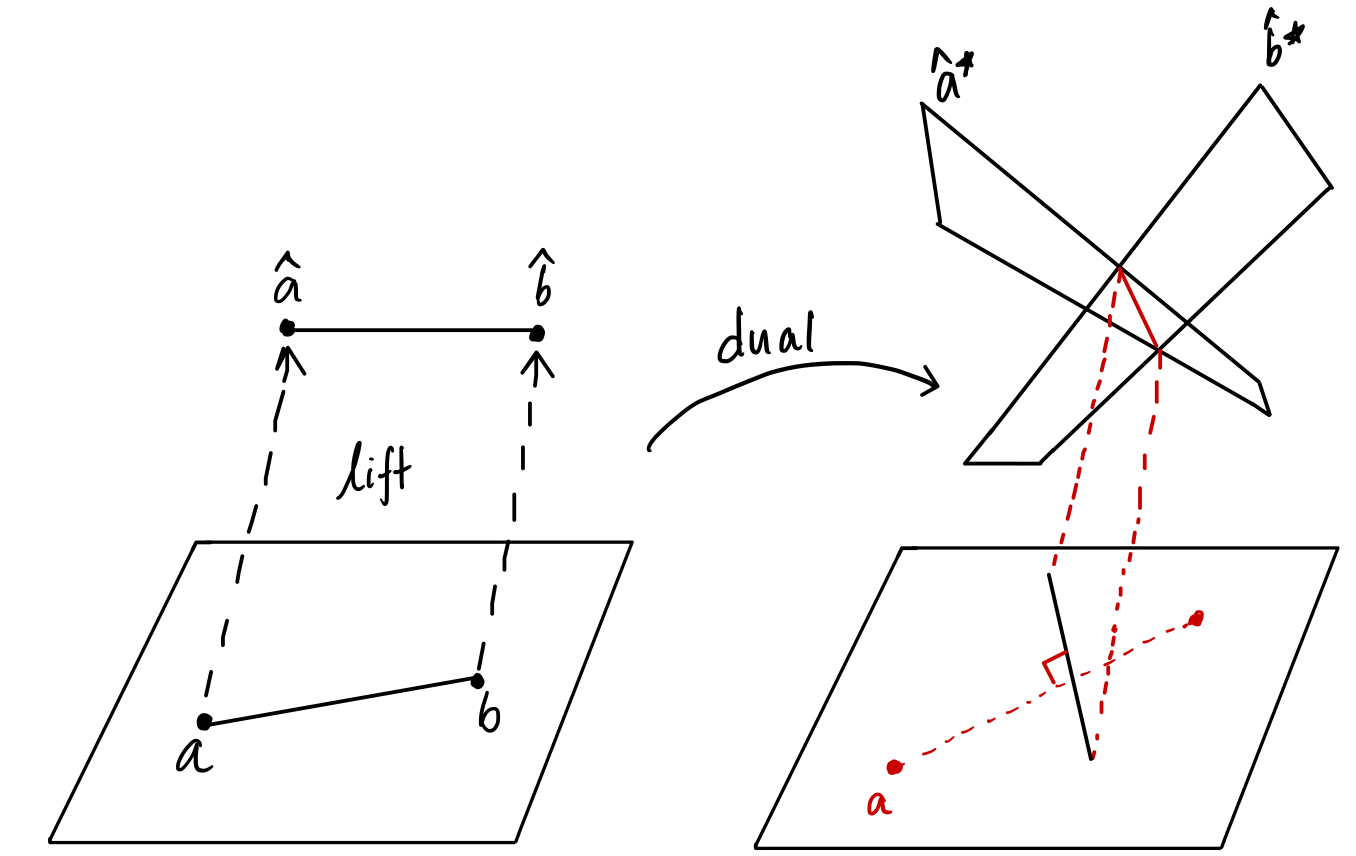
\includegraphics[width=.5\linewidth]{draw_p2.jpeg}
        \caption{The lifting of a $P_2$.}
    \end{figure}
    
    Edges in the primal should be orthogonal to an edge in the dual.
    
    What happens to a $K_3$ after a lifting? Three new planes intersect each other forming a point.
    
    \begin{figure}[H]
        \centering
        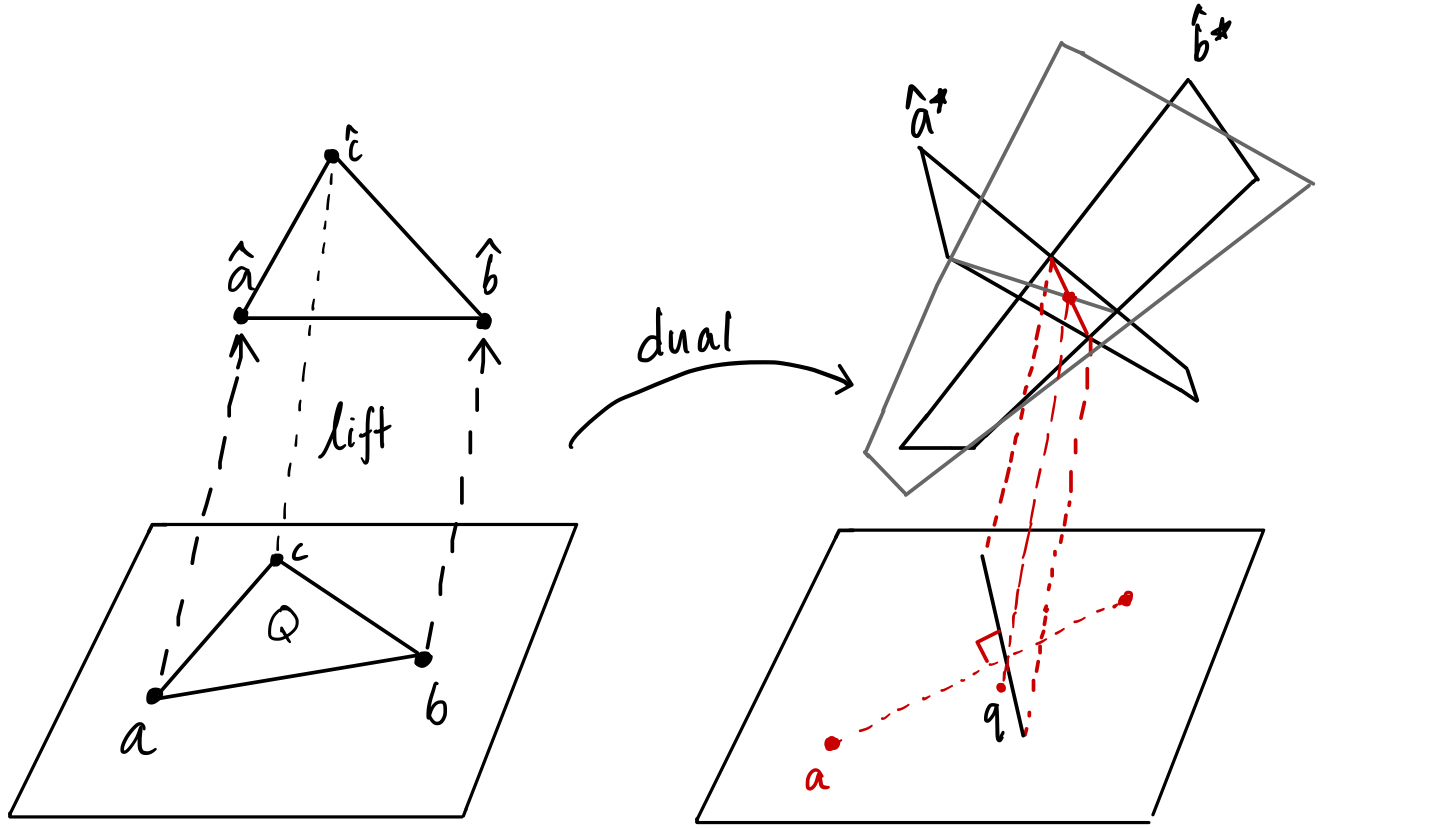
\includegraphics[width=.5\linewidth]{draw_k3.jpeg}
        \caption{The lifting of a $K_3$.}
    \end{figure}
    
    Faces in the primal become a vertex in the dual.
    
    \begin{proposition}
        From the pictures, we hope that $(p-q)^T(a-b) \overset{?}{=}0$ where p, q are primal vertices and a,b are lifted vertices.
    \end{proposition}
    
    \begin{proof}
        In the lifting, 
    
        \begin{align*}
            \hat{p} &\in \hat{a}^* \cap \hat{b}^* \\
            \hat{q} &\in \hat{a}^* \cap \hat{b}^*
        \end{align*}
        
        From the incident formula,
        
        \begin{align*}
            \hat{p}^* &\in \hat{a}^* \Leftrightarrow p_z = a^Tp-a_z \\
            \hat{p}^* &\in \hat{b}^* \Leftrightarrow p_z = b^Tp-b_z \\
            \hat{q}^* &\in \hat{a}^* \Leftrightarrow q_z = a^Tq-a_z \\
            \hat{q}^* &\in \hat{b}^* \Leftrightarrow q_z = b^Tq-b_z \\
        \end{align*}
        
        Rewriting the formulas by transposing both sides,
    
        \begin{align*}
            p_z + a_z &= a^Tp \\
            p_z + a_z &= p^Ta \\ \\
            p_z + b_z &= b^Tp \\
            p_z + b_z &= p^Tb \\ \\
            q_z + a_z &= a^Tq \\
            q_z + a_z &= q^Ta \\ \\
            q_z + b_z &= b^Tq \\
            q_z + b_z &= q^Tb
        \end{align*}
        
        Expanding orthogonality test,
        
        \begin{align*}
            (p-q)^T(a-b) &= p^Ta - q^Ta - p^Tb + q^Tb \\
            &= (p_z + a_z) - (q_z + a_z) - (p_z + b_z) + (q_z + b_z) \\
            &= 0
        \end{align*}
    \end{proof}
    
    \newpage
    
    The correspondences between equilibrium stress and reciprocal diagram, and liftings reciprocal diagrams together implies the Maxwell-Caremona correspondence. 
    
    \begin{figure}[h!]
        \centering
        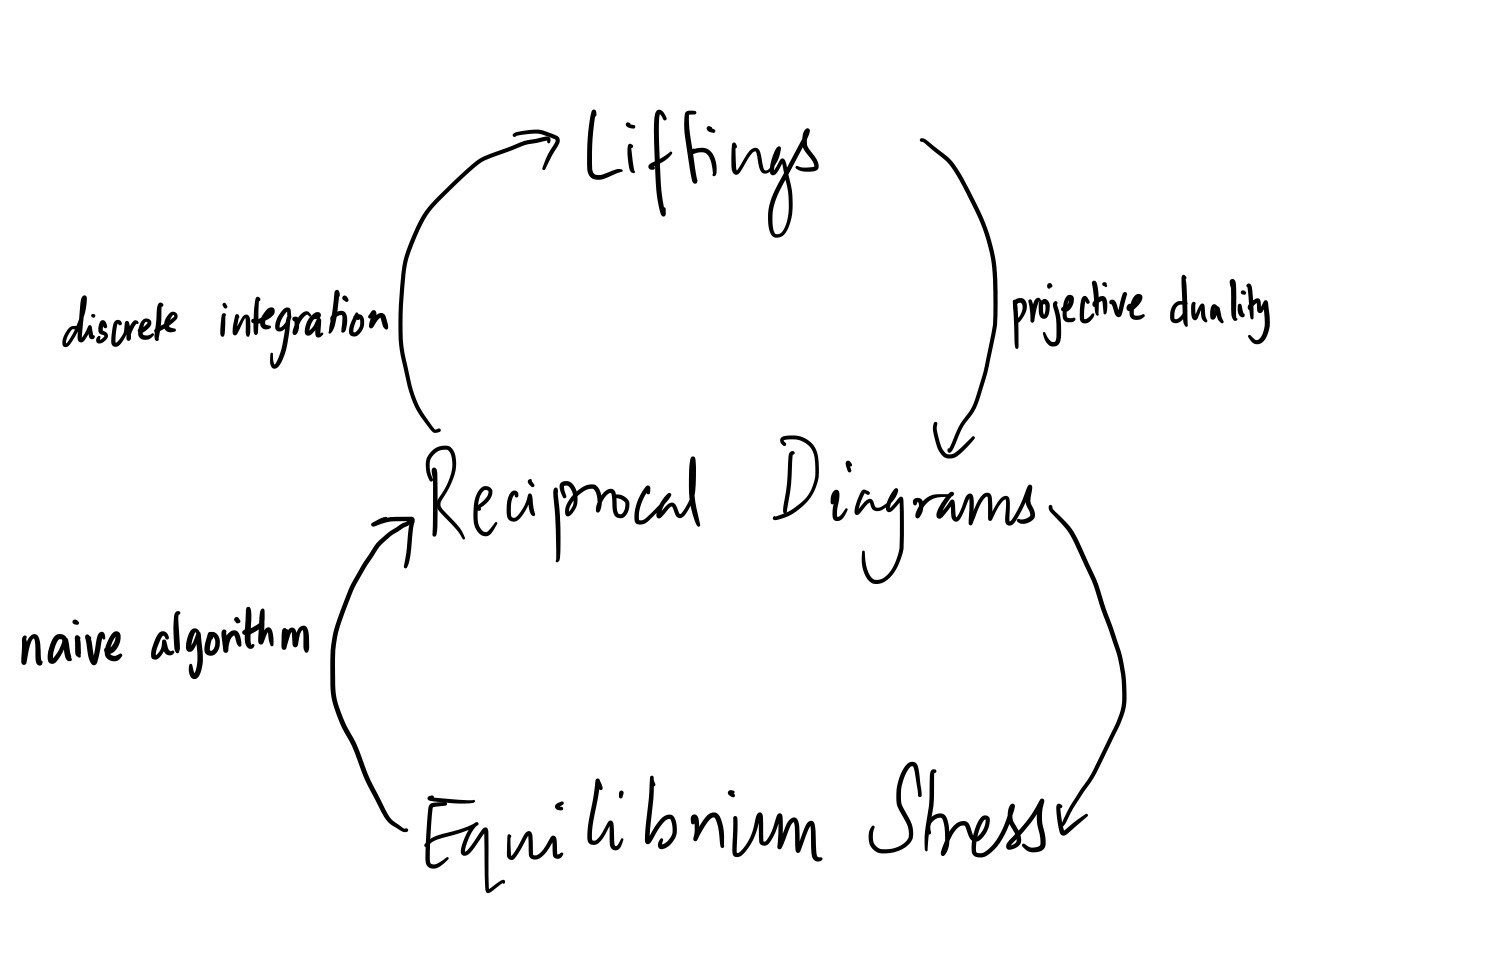
\includegraphics[width=.6\linewidth]{correspondence.JPG}
        \caption{Transformation of objects to different types.}
    \end{figure}
    
    In theory, reciprocal diagrams came from equilibrium. Theoretically, we think of edges in graphs as springs and there is a certain amount of force acting along the edges to keep them in equilibrium. Given a force diagram, where everything is in equilibrium, we draw a polygon for each vertex and glue them together into one diagram, giving us reciprocal diagrams. Figure 13 shows an correspondence between equilibrium stress and reciprocal diagram. 
    
    \begin{figure}[H]
        \centering
        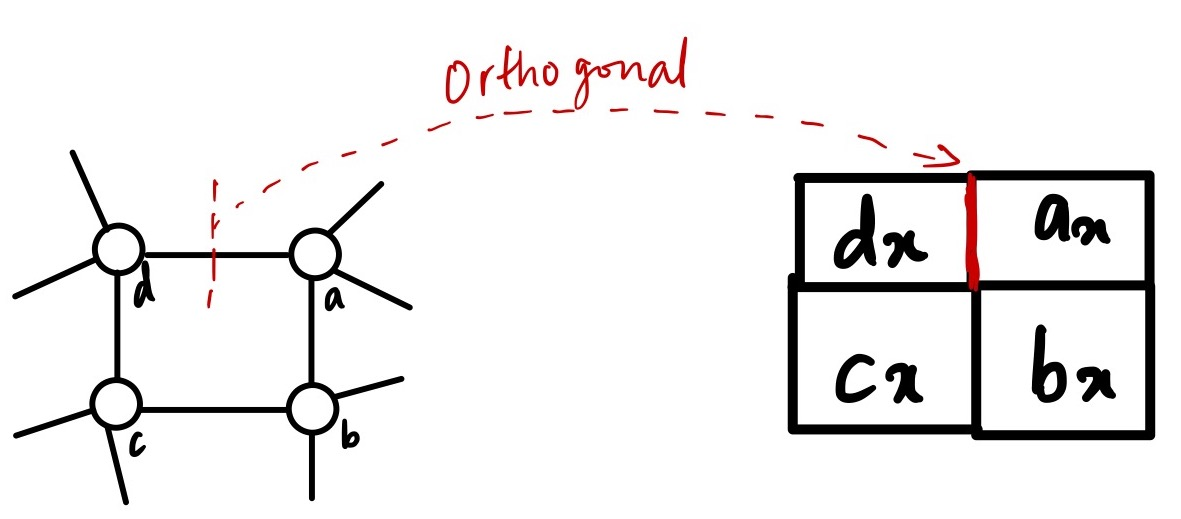
\includegraphics[width=.6\linewidth]{reciprocal-2.JPG}
        \caption{Correspondence between Equilibrium Stress and Reciprocal Diagram}
        \label{fig:reciprocal-corres}
    \end{figure}
    
    One correspondence is seen between liftings and reciprocal diagrams. Given a lifting, you can intuitively get to reciprocal diagrams by projective duality. Look to the planes through every face. Then, those planes in gradient intercept form give the dual vertices for the reciprocal diagram. Similarly, to get a lifting from a reciprocal diagram, the position of every dual vertex can be considered a gradient of the face when it is lifted. We know that gradient of linear form is constant. So, on each face there is a constant gradient. Lifting the faces should be done is a way that the faces match up. The amount of slanting of faces is known but how to lift them is not. So a continuous function is needed in order to glue the faces such that everything is continuous and satisfies the gradient. 
    
    Polyhedron from a graph in plane can be achieved by thinking of \textit{push and pull} forces across the edges of the graph and lifting the graph to make it 3-dimensional. If we are going to lift from a reciprocal diagram, pushing forces will give mountain folds and pulling forces will give valley folds. Figure 14 shows an example of both of the folds.
    
    \begin{figure}[H]
        \centering
        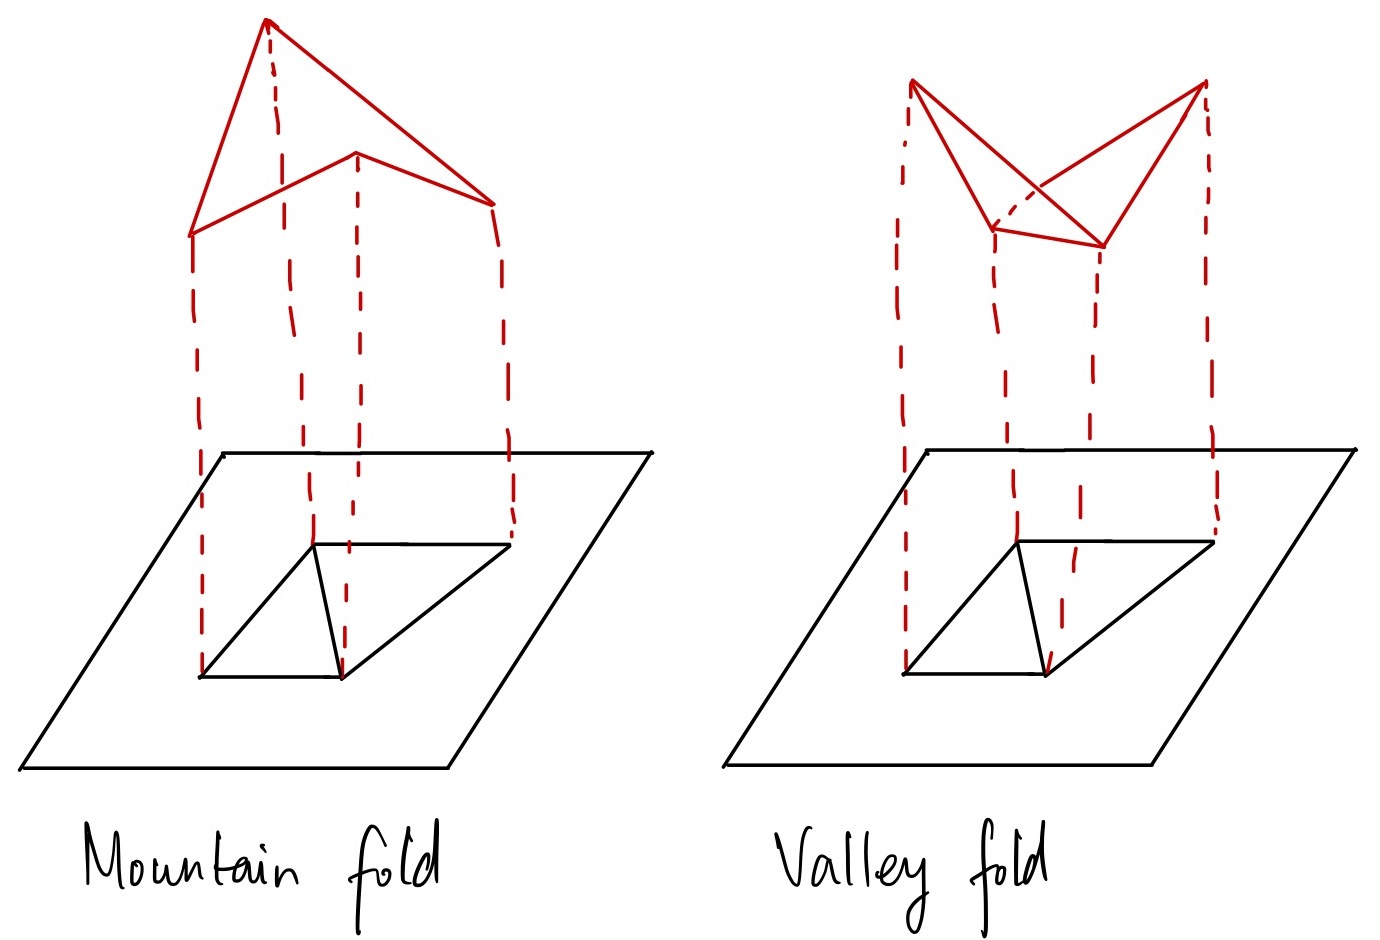
\includegraphics[width=.5\linewidth]{folds.JPG}
        \caption{Mountain and Valley Folds}
        \label{fig:folds}
    \end{figure}
    
    
    Since polyhedra are convex, for the graph to be a polyhedra, the way faces fold after lifting is important. If we want the lifting to be a polyhedron, we want all the folds in the lifting to be either mountain or valley fold. So, for all lifting to be either mountain or valley folds then all the forces needs to be either pulling or pushing forces. However, if all forces are either pulling or pushing forces, then the entire system cannot be in equilibrium. There is a graph drawing algorithm that allows all the forces except the ones corresponding to the outer face can be either pulling or pushing forces. This algorithm is discussed in the next lecture.
    
    
    
    
    
    
\end{document}
